\documentclass[11pt,titlepage]{article}

\usepackage{amsmath,amssymb,amsthm}
\usepackage{booktabs}
\usepackage{tikz}
\usepackage{hyperref}
\usepackage[margin=1in]{geometry}
\usepackage{setspace}
\onehalfspacing

\usepackage[backend=biber, style=apa]{biblatex}
\DeclareLanguageMapping{english}{english-apa}
\addbibresource{synchronization.bib}

\newtheorem{theorem}{Theorem}
\newtheorem{lemma}[theorem]{Lemma}
\newtheorem{corollary}[theorem]{Corollary}
\newtheorem{proposition}[theorem]{Proposition}
\newtheorem{definition}[theorem]{Definition}
\newtheorem{remark}[theorem]{Remark}
\newtheorem{conjecture}[theorem]{Conjecture}

\title{Permutation-Schedule Dominance for Two-Stage Assembly\\
  Flow Shops with Divisible Work}

\author{Eric Bowman\\
  \small King, Berlin, Germany\\
  \small \texttt{eric.bowman@king.com}\\
  \small ORCID: 0009-0003-9171-7217}

\date{}

\begin{document}

\maketitle

\begin{abstract}
Permutation schedules are known to dominate in the classical
two-stage assembly flow shop for makespan and weighted completion time.
We extend this dominance property to a divisible-work model in
which each stage-1 machine contains $k$ identical parallel
workers, job workloads may differ by machine, and work is
allocated integrally across workers. The proof rests on a
three-step logical chain. First, a capacity bound establishes
that $k$ workers can complete at most $kt$ units of work by
time~$t$, limiting the total work completable before any
deadline. Second, a water-filling allocation that balances
worker loads achieves this bound with equality (up to an
integer ceiling), so the constructed permutation schedule
meets every release-time deadline set by the original schedule.
Third, because release times do not increase, the max-plus
recurrence at stage~2 yields pointwise domination:
$C^{(2)}_j(S^*) \leq C^{(2)}_j(S)$ for every job~$j$.
This implies optimality of permutation schedules for every
regular stage-2 objective, including makespan, total weighted
completion time, and maximum lateness. The result extends to
instances where each job visits only a subset of stage-1
machines. The classical model is recovered when $k = 1$.
Small instances are exhaustively verified computationally,
and the core arguments are formalized in Lean~4.
We systematically map the boundaries of this dominance:
it extends to two-stage chains but fails for chains of
length $L \geq 3$, where we identify the precise failure
mechanism. Computational evidence across over $20$ million
instances characterizes behavior for wider DAG topologies.
\end{abstract}

\noindent\textbf{Keywords:} assembly flow shop; permutation
schedule; divisible work; weighted completion time; scheduling
theory

\noindent\textbf{Mathematics Subject Classification:} 90B35

%% ============================================================
\section{Introduction}
\label{sec:intro}

The two-stage assembly flow shop, introduced by
\textcite{lee1993}, consists of $m$ parallel machines at
stage~1, each processing all $n$~jobs without preemption,
followed by a single assembly machine at stage~2 that can begin
job~$j$ only after all stage-1 machines have completed~$j$.

\textcite{potts1995} proved the problem is NP-hard
for $m \geq 2$ and that \emph{permutation schedules
dominate}: the search for a $C_{\max}$-optimal schedule may be
restricted to schedules where all stage-1 machines use the same
job ordering, reducing the search space from $(n!)^m$ orderings
to~$n!$. \textcite{tozkapan2003}
extended permutation-schedule dominance to the total
weighted completion-time objective.
\textcite{hariri1997} developed
a branch-and-bound algorithm with dominance theorems,
testing on instances with up to $n = 8000$ jobs and $m = 10$ machines. \textcite{hadda2024} contributed new dominance rules
and an exact branch-and-bound, solving instances up to
$n = 1000$, $m = 8$.

\textcite{koulamas2007} studied a variant
with \emph{uniform} parallel machines at stage~1 (machines with
different speeds). Their model differs from ours: uniform
machines have one processor per machine at varying speeds,
whereas our model has $k$ identical workers per machine sharing
divisible work.

We distinguish several adjacent lines of work. The malleable-job
literature \parencite{drozdowski2009} studies divisible
work on parallel processors but without the assembly constraint.
\textcite{alanzi2007} study the two-stage
assembly problem with setup times, using permutation dominance
to restrict the heuristic search space. \textcite{hatami2013} consider distributed assembly
permutation flow shops (multiple factories, not multiple workers
per machine). \textcite{zhang2022} study assembly
scheduling with parallel teams and heterogeneous worker skills,
in a multi-objective setting without dominance results. \textcite{komaki2019} survey assembly flow
shop models; the divisible-work model studied here does not
appear in their taxonomy. \textcite{framinan2019} provide a comprehensive
classification of concurrent-type assembly scheduling models,
complementing the survey of Komaki et al.
\textcite{fv2022} develop
speed-up procedures for insertion-based heuristics for the
classical assembly flow shop, proving theoretical properties
of the problem structure. These recent contributions address
algorithmic and computational aspects of the classical model
but do not establish dominance results for the divisible-work
generalization.

To the best of our knowledge, the divisible-work assembly
flow shop model --- combining the assembly constraint with
team-based parallel workers sharing divisible work --- has not
been studied previously, and the dominance result proved here
is new.

In modern enterprise software engineering, cross-functional delivery
frequently relies on parallel build phases (backend, frontend, platform
teams) followed by a strict integration phase --- precisely the
fork-join structure captured by the assembly flow shop.  When teams
independently optimise their own orderings, delivery stalls arise not
from capacity shortages but from misaligned sequencing: one team
completes its portion of an initiative while another has not yet
started, leaving work blocked at the integration barrier.

While permutation-schedule dominance is highly desirable, a natural
theoretical question is how far this property extends beyond the
two-stage assembly topology. We conduct a systematic boundary
investigation, proving that dominance extends to two-stage chains
(Theorem~\ref{thm:chain-l2}) but fails for longer chains
(Proposition~\ref{prop:chain-failure}), and providing extensive
computational evidence for wider DAG structures. The complete
dominance landscape is summarized in Table~\ref{tab:landscape}.

\subsection{Contribution}

We prove that permutation-schedule dominance extends to a
divisible-work generalization where each stage-1 machine has
$k \geq 1$ identical parallel workers and work requirements
$w_{i,j}$ may differ across machines. Setting $k = 1$ recovers
the classical model. The specific contributions are:
\begin{enumerate}
  \item The extension from $k = 1$ to $k \geq 1$ workers per
        machine with integer work division, including the case
        $d_{i,j,\ell} \geq 0$ (some workers idle) and
        $w_{i,j} \geq 0$ (jobs may skip machines).
  \item Machine-dependent work requirements $w_{i,j}$.
  \item A constructive proof avoiding pairwise exchanges,
        unlike the exchange-argument technique of
        \textcite{potts1995}. Their proof transforms a schedule
        by pairwise job exchanges, tracking the assembly barrier
        at each step; ours constructs the permutation schedule
        directly from a single inequality without intermediate
        exchanges. The construction requires $O(n \log n)$
        time to sort jobs by release time and $O(nk)$ time
        per machine for water-filling (each job's work is
        distributed in $O(k)$ time by batched
        floor-and-remainder allocation), giving
        $O(n \log n + mnk)$ overall.
\end{enumerate}

\noindent
The reduction from $(n!)^m$ to $n!$ has practical significance
beyond computational tractability: when teams independently optimise
their own orderings, the resulting schedule can be significantly
suboptimal.  The magnitude of this ``cost of independent
prioritisation'' is quantified computationally in
Section~\ref{sec:computation}.

%% ============================================================
\section{Model}
\label{sec:model}

\begin{definition}[Divisible-Work Two-Stage Assembly Flow Shop]
\label{def:model}
An instance consists of:
\begin{itemize}
  \item $n$ jobs, indexed $j \in [n] = \{1, \ldots, n\}$.
  \item $m$ stage-1 machines, each with $k$ identical workers
        ($k \geq 1$).
  \item One stage-2 assembly machine. Stage~2 can begin
        job~$j$ only after all stage-1 machines have
        completed~$j$; it then processes~$j$ for
        $q_j \in \mathbb{Z}_{> 0}$ time units.
  \item Work requirements $w_{i,j} \in \mathbb{Z}_{\geq 0}$ for
        each machine $i \in [m]$ and job $j \in [n]$. When
        $w_{i,j} = 0$, job~$j$ does not require machine~$i$;
        machine~$i$ does not constrain~$r_j$.
\end{itemize}
\end{definition}

\noindent
The integer work requirements $w_{i,j} \in \mathbb{Z}_{\geq 0}$
model atomic task units common in practice --- person-days, story
points, or discrete manufacturing batches --- where partial units
cannot be meaningfully assigned.

\begin{definition}[Schedule]
\label{def:schedule}
A schedule $S = (\boldsymbol{\sigma}, \mathbf{d}, \tau)$
consists of:
\begin{itemize}
  \item Permutations $\sigma_i \in \mathfrak{S}_n$ for each
        machine $i$: machine~$i$ processes jobs in order
        $\sigma_i(1), \ldots, \sigma_i(n)$.
  \item Work divisions $d_{i,j,\ell} \in \mathbb{Z}_{\geq 0}$
        for each machine $i$, job $j$, worker $\ell \in [k]$,
        satisfying $\sum_{\ell} d_{i,j,\ell} = w_{i,j}$.
  \item A permutation $\tau \in \mathfrak{S}_n$ giving the
        stage-2 processing order.
\end{itemize}
The work division $\mathbf{d}$ is determined \emph{before}
execution begins: it specifies, for each machine~$i$ and
job~$j$, how many units each worker~$\ell$ will process.
All processing is non-preemptive: each worker processes
its assigned portion $d_{i,j,\ell}$ of a job as a single
contiguous block before starting the next job in the
permutation order. When $d_{i,j,\ell} = 0$, worker~$\ell$
performs no work on job~$j$ and is available for the next
job immediately.
\end{definition}

\begin{definition}[Completion Times]
\label{def:completion}
Worker $\ell$ on machine $i$ processes jobs sequentially in
order $\sigma_i$. The cumulative finish time after position $s$
is $F_{i,\ell,s} = \sum_{t=1}^{s} d_{i,\sigma_i(t),\ell}$.
The \emph{completion time} of job $j$ on machine~$i$ is the
time at which all workers who contribute to~$j$ have finished:
\[
  C_{i,j} \;=\; \max_{\ell :\, d_{i,j,\ell} > 0}
  F_{i,\ell,\,\sigma_i^{-1}(j)}.
\]
When $w_{i,j} = 0$ (so every $d_{i,j,\ell} = 0$), we set
$C_{i,j} = 0$.

The \emph{release time} of job $j$ to stage~2 is
$r_j = \max_{i \in [m]} C_{i,j}$.

Stage~2 processes jobs non-preemptively in order $\tau$ on
a single machine. The stage-2 completion time of job
$\tau(s)$ is given by the max-plus recurrence
\[
  C^{(2)}_{\tau(s)} \;=\; \max\!\big(C^{(2)}_{\tau(s-1)},\;
  r_{\tau(s)}\big) + q_{\tau(s)},
\]
with $C^{(2)}_{\tau(0)} := 0$.
The makespan is $C_{\max}(S) = C^{(2)}_{\tau(n)}$.
\end{definition}

\begin{definition}[Permutation Schedule]
A schedule is a \emph{permutation schedule} if
$\sigma_1 = \sigma_2 = \cdots = \sigma_m$.
\end{definition}

In the three-field notation of
\textcite{graham1979}, the problem is
$\text{FH2}(P_{m \times k}, 1) \mid
\text{assembly, div} \mid C_{\max}$, where ``div'' denotes
divisible integer work.

%% ============================================================
\section{Main Result}
\label{sec:main}

\begin{theorem}[Pointwise Stage-2 Domination]
\label{thm:main}
For every feasible schedule $S$, there exists a permutation
schedule $S^*$ --- whose permutation depends on the release
times of $S$ --- such that
$C^{(2)}_j(S^*) \leq C^{(2)}_j(S)$ for every job~$j$.
\end{theorem}

\begin{corollary}
\label{cor:main}
Permutation schedules are optimal for every regular
(non-decreasing) function of stage-2 completion times,
including $C_{\max}$, $\sum_j v_j C^{(2)}_j$ for any
$v_j > 0$, and $\max_j (C^{(2)}_j - \bar{d}_j)$ for any due
dates~$\bar{d}_j$.
\end{corollary}

The proof of Theorem~\ref{thm:main} uses two lemmas. The
assembly constraint --- stage~2 cannot begin job~$j$ until
every stage-1 machine has finished --- is captured by a single
capacity inequality, from which the construction follows.

\begin{lemma}[Capacity Bound]
\label{lem:capacity}
Let $S$ be any schedule with release times $r_j$. Let $\pi$ be
any permutation sorting jobs by non-decreasing release time:
$r_{\pi(1)} \leq \cdots \leq r_{\pi(n)}$ (ties broken
arbitrarily). Then for every machine $i$ and every
$s \in [n]$:
\[
  W_i(s) \;:=\; \sum_{t=1}^{s} w_{i,\pi(t)}
  \;\leq\; k \cdot r_{\pi(s)}.
\]
\end{lemma}

\begin{proof}
In schedule $S$, machine $i$ completes job $\pi(t)$ by time
$C_{i,\pi(t)} \leq r_{\pi(t)} \leq r_{\pi(s)}$ for each
$t \leq s$. Hence by time $r_{\pi(s)}$, machine $i$ has
completed all jobs in $\{\pi(1), \ldots, \pi(s)\}$, whose
total work is $W_i(s)$. Since $k$ workers each contribute at
most $r_{\pi(s)}$ time units: $W_i(s) \leq k \cdot r_{\pi(s)}$.
\end{proof}

\begin{lemma}[Water-Filling Feasibility]
\label{lem:waterfill}
Given machine $i$ processing jobs in order $\pi$, water-filling
--- assigning integer portions of each job's work so that
cumulative worker loads remain as balanced as possible ---
produces a valid non-preemptive work division with
$\sum_\ell d_{i,\pi(s),\ell} = w_{i,\pi(s)}$ and achieves
\[
  C^*_{i,\pi(s)} \;\leq\; \lceil W_i(s) / k \rceil
  \qquad\text{for each position } s.
\]
\end{lemma}

\begin{proof}
We prove a load-balancing invariant, then derive the
completion-time bound.

\medskip\noindent\textbf{Load balancing.}
By induction on $s$. The invariant: after allocating work for
position $s$, the cumulative load of each worker $\ell$ ---
namely $F_{i,\ell,s} = \sum_{t=1}^{s} d_{i,\pi(t),\ell}$ ---
lies in
$\{\lfloor W_i(s)/k \rfloor, \lceil W_i(s)/k \rceil\}$.
That is, loads differ by at most~1 and sum to $W_i(s)$.

\emph{Base case} ($s = 0$): all loads are zero.

\emph{Inductive step}: at position $s$, distribute
$w_{i,\pi(s)}$ units one at a time, each to a currently
least-loaded worker. Since the invariant holds at $s{-}1$,
loads before allocation differ by at most~1. Adding units
one-at-a-time to the minimum maintains the spread $\leq 1$:
each unit either raises a minimum-load worker to the current
maximum, or (once all workers are equal) raises all loads
uniformly. The cumulative total becomes $W_i(s)$, so the
maximum worker load is $\lceil W_i(s)/k \rceil$.

When $w_{i,\pi(s)} \geq k$, every worker receives at least one
unit. When $w_{i,\pi(s)} < k$, some workers are idle for this
job ($d_{i,\pi(s),\ell} = 0$).

\medskip\noindent\textbf{Completion-time bound.}
By Definition~\ref{def:completion},
$C^*_{i,\pi(s)} = \max_{\ell:\,d_{i,\pi(s),\ell}>0}
F_{i,\ell,s}$.
Every worker who contributes to job $\pi(s)$ has cumulative
load $F_{i,\ell,s} \leq \lceil W_i(s)/k \rceil$ by the
invariant. Hence
$C^*_{i,\pi(s)} \leq \lceil W_i(s)/k \rceil$.

\medskip\noindent\textbf{Non-preemptive feasibility.}
Worker $\ell$ processes jobs in the fixed order $\pi$:
for each $s = 1, \ldots, n$, the worker executes its
$d_{i,\pi(s),\ell}$ units as a single contiguous block
(taking zero time when $d_{i,\pi(s),\ell} = 0$). Since the
job order is the same for all workers and each worker processes
its portion without interruption, the schedule is
non-preemptive in the sense of Definition~\ref{def:schedule}.
\end{proof}

\begin{proof}[Proof of Theorem~\ref{thm:main}]
Given schedule $S$ with release times $r_j$, let $\pi$ sort
jobs by non-decreasing $r_j$. Construct $S^*$:
\begin{enumerate}
  \item Every stage-1 machine uses permutation $\pi$.
  \item Each machine $i$ independently uses water-filling
        (Lemma~\ref{lem:waterfill}) to allocate $w_{i,\pi(s)}$.
  \item Stage~2 uses the same order $\tau$ as $S$.
\end{enumerate}

By Lemma~\ref{lem:waterfill},
$C^*_{i,\pi(s)} \leq \lceil W_i(s)/k \rceil$.
By Lemma~\ref{lem:capacity}, $W_i(s) \leq k \cdot r_{\pi(s)}$.
Since $r_{\pi(s)}$ is a non-negative integer:
$\lceil W_i(s)/k \rceil \leq r_{\pi(s)}$ for all $i, s$.
Therefore $r^*_j \leq r_j$ for all~$j$.

Since $r^*_j \leq r_j$ and stage~2 uses the same order $\tau$,
the max-plus recurrence gives, by induction on positions:
$C^{(2)}_{\tau(s)}(S^*) \leq C^{(2)}_{\tau(s)}(S)$ for all~$s$.
Therefore $C^{(2)}_j(S^*) \leq C^{(2)}_j(S)$ for every~$j$.
The construction requires $O(n \log n)$ time to sort and
$O(nk)$ per machine for water-filling---each job with work~$w$
assigns $\lfloor w/k \rfloor$ to every worker and distributes
the $w \bmod k$ remainder one-per-worker among the
minimum-load workers in $O(k)$ time, preserving the invariant
that loads differ by at most~$1$---giving
$O(n \log n + mnk)$ overall.
\end{proof}

\begin{remark}[Classical recovery]
When $k = 1$, water-filling is the identity and the theorem
recovers the permutation-schedule dominance of
\textcite{potts1995}.
\end{remark}

\begin{remark}[Existential nature and scope]
\label{rem:existential}
The result is a \emph{dominance} statement, not a claim of
global optimality over all permutations. The constructed
permutation $\pi$ depends on the release times of the given
schedule~$S$; different schedules may yield different
permutations. Theorem~\ref{thm:main} asserts that for every
feasible schedule, \emph{some} permutation schedule is at
least as good pointwise. It does not identify which
permutation is globally optimal --- that remains NP-hard.
\end{remark}

\begin{remark}[Stage-2 monotonicity]
\label{rem:stage2}
The final step uses a standard property of the max-plus
recurrence: if $r^*_j \leq r_j$ for all~$j$ and the stage-2
order is held fixed, then $C^{(2)}_j(S^*) \leq C^{(2)}_j(S)$
for all~$j$. This holds immediately by induction for the
classical single-machine stage~2 defined above. The result
extends to any stage-2 model whose completion times are
monotone non-decreasing in release times, but does not extend
to models with sequence-dependent setup times or blocking
constraints where this monotonicity may fail.
\end{remark}

\begin{remark}[Tie-breaking in $\pi$]
\label{rem:ties}
When multiple jobs share the same release time, any
tie-breaking order suffices. The capacity bound
(Lemma~\ref{lem:capacity}) holds for all orderings
consistent with non-decreasing release times, since it
depends only on the set of jobs completed by each time
point, not on the ordering within a tie class.
\end{remark}

\begin{remark}[Integrality]
\label{rem:integrality}
The model assumes integer work requirements
$w_{i,j} \in \mathbb{Z}_{\geq 0}$ and integer work
divisions. The ceiling in the water-filling bound is needed
when $w_{i,j} \geq 1$ on machines that process the job. In a continuous model (rational
or real-valued work, arbitrary division), water-filling
achieves exact balance $W_i(s)/k$ at each position, and
the ceiling becomes an equality. The dominance result
therefore holds \emph{a fortiori} in the continuous case.
\end{remark}

\begin{remark}[Job-dependent machine subsets]
\label{rem:subsets}
Since $w_{i,j} \geq 0$ (Definition~\ref{def:model}), the
model accommodates jobs that visit only a subset
$S_j = \{i : w_{i,j} > 0\} \subseteq [m]$ of stage-1
machines. Machine~$i$ processes only jobs in
$J_i = \{j : w_{i,j} > 0\}$. The capacity bound
(Lemma~\ref{lem:capacity}) holds on $J_i$: the cumulative
work $W_i(s)$ sums only over jobs in $J_i$ completed by
time~$r_{\pi(s)}$, and the $k$ workers contribute at most
$k \cdot r_{\pi(s)}$ units regardless of which jobs they
process. Water-filling (Lemma~\ref{lem:waterfill}) applies
to the restricted subsequence. The proof is unchanged:
$r^*_j = \max_{i \in S_j} C^*_{i,j} \leq r_j$.
\end{remark}

\begin{remark}[Stage-2 re-optimization]
The construction inherits the stage-2 order $\tau$ unchanged.
Re-optimizing $\tau$ for the improved release times can only
improve the result but is not needed for dominance.
\end{remark}

\paragraph{Example.}
Let $n = 3$, $m = 2$, $k = 2$. Machine~1: $(w_{1,A},
w_{1,B}, w_{1,C}) = (6, 4, 2)$; machine~2: $(w_{2,A},
w_{2,B}, w_{2,C}) = (2, 6, 4)$.

Schedule $S$: machine~1 uses $A, B, C$; machine~2 uses
$B, C, A$. Water-filling gives: machine~1 completes $A$ at~3,
$B$ at~5, $C$ at~6; machine~2 completes $B$ at~3, $C$ at~5,
$A$ at~6. Release times: $r_A = 6$, $r_B = 5$, $r_C = 6$.

Sort: $\pi = (B, A, C)$. Capacity bound holds:
$W_1(1) = 4 \leq 10$, $W_2(1) = 6 \leq 10$, etc.
Water-filling with $\pi$: $r^*_B = 3 \leq 5$,
$r^*_A = 5 \leq 6$, $r^*_C = 6 \leq 6$.
Figure~\ref{fig:example} shows the two schedules side by side.

\begin{figure}[ht]
\centering
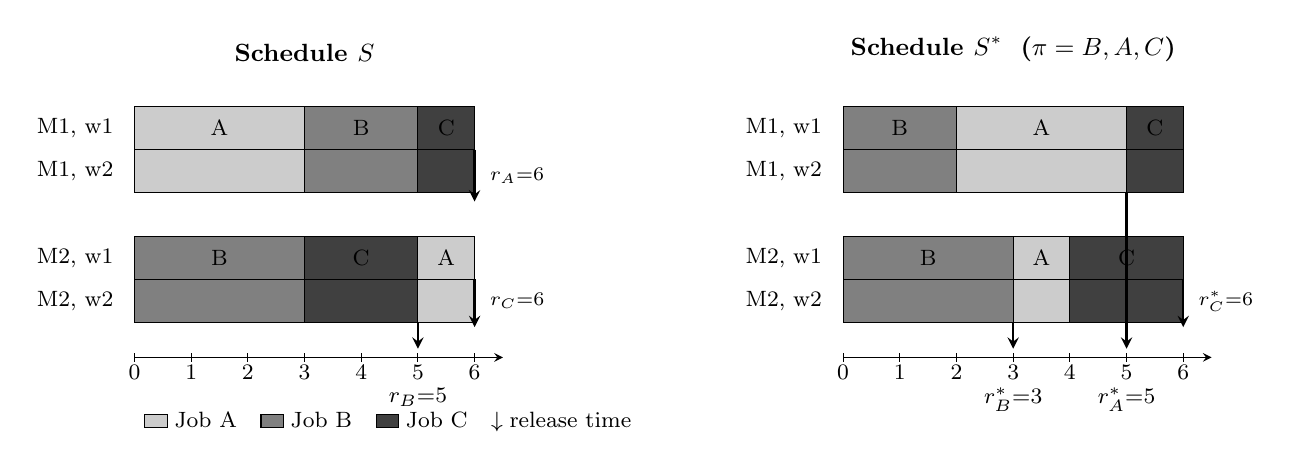
\begin{tikzpicture}[
    x=0.72cm, y=0.55cm,
    jobA/.style={fill=black!20},
    jobB/.style={fill=black!50},
    jobC/.style={fill=black!75},
    >=stealth,
    font=\footnotesize
  ]

  %% ---- Left: Schedule S (unsynchronized) ----
  \node[anchor=south, font=\small\bfseries] at (3,5.8) {Schedule $S$};

  % Machine 1 label
  \node[anchor=east] at (-0.2,4.5) {M1, w1};
  \node[anchor=east] at (-0.2,3.5) {M1, w2};

  % Machine 1, worker 1: A(3), B(2), C(1) => A:0-3, B:3-5, C:5-6
  \draw[jobA] (0,4) rectangle (3,5);
  \draw[jobB] (3,4) rectangle (5,5);
  \draw[jobC] (5,4) rectangle (6,5);
  % Machine 1, worker 2: A(3), B(2), C(1) => A:0-3, B:3-5, C:5-6
  \draw[jobA] (0,3) rectangle (3,4);
  \draw[jobB] (3,3) rectangle (5,4);
  \draw[jobC] (5,3) rectangle (6,4);

  % Machine 2 label
  \node[anchor=east] at (-0.2,1.5) {M2, w1};
  \node[anchor=east] at (-0.2,0.5) {M2, w2};

  % Machine 2, order B,C,A: B(3),C(2),A(1) => B:0-3, C:3-5, A:5-6
  \draw[jobB] (0,1) rectangle (3,2);
  \draw[jobC] (3,1) rectangle (5,2);
  \draw[jobA] (5,1) rectangle (6,2);
  % Machine 2, worker 2: B(3),C(2),A(1)
  \draw[jobB] (0,0) rectangle (3,1);
  \draw[jobC] (3,0) rectangle (5,1);
  \draw[jobA] (5,0) rectangle (6,1);

  % Job labels inside blocks
  \node at (1.5,4.5) {A};
  \node at (4,4.5) {B};
  \node at (5.5,4.5) {C};
  \node at (1.5,1.5) {B};
  \node at (4,1.5) {C};
  \node at (5.5,1.5) {A};

  % Time axis
  \draw[->] (0,-0.8) -- (6.5,-0.8);
  \foreach \t in {0,1,...,6} \draw (\t,-0.9) -- (\t,-0.7) node[below,yshift=-1pt]{\t};

  % Release time arrows (max completion across machines)
  % r_B = max(5,3) = 5
  \draw[->,thick] (5,0) -- (5,-0.6);
  \node[anchor=north,yshift=-6pt] at (5,-0.9) {$r_B{=}5$};
  % r_A = max(3,6) = 6
  \draw[->,thick] (6,4) -- (6,2.8);
  \node[anchor=west,font=\scriptsize] at (6.1,3.4) {$r_A{=}6$};
  % r_C = max(6,5) = 6
  \draw[->,thick] (6,1) -- (6,-0.1);
  \node[anchor=west,font=\scriptsize] at (6.1,0.5) {$r_C{=}6$};

  %% ---- Right: Schedule S* (synchronized, pi=(B,A,C)) ----
  \begin{scope}[xshift=9cm]
  \node[anchor=south, font=\small\bfseries] at (3,5.8) {Schedule $S^*$\; ($\pi = B, A, C$)};

  % Machine 1 label
  \node[anchor=east] at (-0.2,4.5) {M1, w1};
  \node[anchor=east] at (-0.2,3.5) {M1, w2};

  % Machine 1, order B,A,C: B(2),A(3),C(1) => B:0-2, A:2-5, C:5-6
  \draw[jobB] (0,4) rectangle (2,5);
  \draw[jobA] (2,4) rectangle (5,5);
  \draw[jobC] (5,4) rectangle (6,5);
  % Machine 1, worker 2
  \draw[jobB] (0,3) rectangle (2,4);
  \draw[jobA] (2,3) rectangle (5,4);
  \draw[jobC] (5,3) rectangle (6,4);

  % Machine 2 label
  \node[anchor=east] at (-0.2,1.5) {M2, w1};
  \node[anchor=east] at (-0.2,0.5) {M2, w2};

  % Machine 2, order B,A,C: B(3),A(1),C(2) => B:0-3, A:3-4, C:4-6
  \draw[jobB] (0,1) rectangle (3,2);
  \draw[jobA] (3,1) rectangle (4,2);
  \draw[jobC] (4,1) rectangle (6,2);
  % Machine 2, worker 2
  \draw[jobB] (0,0) rectangle (3,1);
  \draw[jobA] (3,0) rectangle (4,1);
  \draw[jobC] (4,0) rectangle (6,1);

  % Job labels inside blocks
  \node at (1,4.5) {B};
  \node at (3.5,4.5) {A};
  \node at (5.5,4.5) {C};
  \node at (1.5,1.5) {B};
  \node at (3.5,1.5) {A};
  \node at (5,1.5) {C};

  % Time axis
  \draw[->] (0,-0.8) -- (6.5,-0.8);
  \foreach \t in {0,1,...,6} \draw (\t,-0.9) -- (\t,-0.7) node[below,yshift=-1pt]{\t};

  % Release time arrows
  % r*_B = max(2,3) = 3
  \draw[->,thick] (3,0) -- (3,-0.6);
  \node[anchor=north,yshift=-6pt] at (3,-0.9) {$r^*_B{=}3$};
  % r*_A = max(5,4) = 5
  \draw[->,thick] (5,3) -- (5,-0.6);
  \node[anchor=north,yshift=-6pt] at (5,-0.9) {$r^*_A{=}5$};
  % r*_C = max(6,6) = 6
  \draw[->,thick] (6,1) -- (6,-0.1);
  \node[anchor=west,font=\scriptsize] at (6.1,0.5) {$r^*_C{=}6$};

  \end{scope}

  %% Legend
  \node[anchor=west] at (0,-2.3) {%
    \tikz{\draw[jobA] (0,0) rectangle (0.4,0.3);}\;Job A\quad
    \tikz{\draw[jobB] (0,0) rectangle (0.4,0.3);}\;Job B\quad
    \tikz{\draw[jobC] (0,0) rectangle (0.4,0.3);}\;Job C\quad
    $\downarrow$\;release time};

\end{tikzpicture}
\caption{Worked example: unsynchronized schedule $S$ (left) vs.\
synchronized schedule $S^*$ (right). Each machine has $k=2$
workers shown as two rows. Release times improve or stay equal
for every job: $r^*_B = 3 \leq 5 = r_B$, $r^*_A = 5 \leq 6 = r_A$,
$r^*_C = 6 \leq 6 = r_C$.}
\label{fig:example}
\end{figure}

%% ============================================================
\section{Computational Verification and Lean~4 Formalization}
\label{sec:computation}

We verified Theorem~\ref{thm:main} by exhaustive enumeration
across 27 homogeneous-work configurations ($w_{i,j} = w_j$;
3,846,136 schedules) and 12 heterogeneous-work configurations
($w_{i,j}$ varying across machines; 167,120 schedules), with
$n \in \{2,3,4,5\}$, $m \in \{2,3\}$, $k \in \{2,3\}$.
The homogeneous configurations include symmetric work
($w_j$ equal for all~$j$), asymmetric work ($w_j$ varying
across jobs), and value-weighted variants (with non-uniform
$v_j > 0$) to test the weighted completion-time objective.
For every schedule~$S$ in every configuration, the
construction of Theorem~\ref{thm:main} produced a permutation
schedule~$S^*$ satisfying $C^{(2)}_j(S^*) \leq C^{(2)}_j(S)$
for every job~$j$ --- i.e., pointwise stage-2 domination was
verified exhaustively.

Beyond verifying dominance, we quantified the practical cost of
independent prioritisation.  Across thousands of random
configurations with $n \in \{3, \ldots, 8\}$,
$m \in \{2, 3, 4\}$, $k \in \{2, 3\}$, and work values drawn
uniformly from $\{1, \ldots, 6\}$, a randomly chosen permutation
schedule achieves equal or better makespan than a randomly chosen
independent schedule in $96$--$99.9\%$ of instances, with an
average makespan improvement of $17$--$29\%$.  This gap widens
with~$n$, reflecting the combinatorial explosion of misalignment
opportunities as the number of jobs grows.  These figures compare
two equally imperfect selection processes; locally optimised
independent orderings would narrow the gap, but cannot eliminate
it by Theorem~\ref{thm:main}.

The dominance argument and the water-filling feasibility
argument (Theorem~\ref{thm:main}) are formalized in Lean~4
(v4.29.0, Mathlib) with zero unresolved
axioms.\footnote{Source code, verification data, and Lean
formalization: \url{https://github.com/ebowman/prioritizer}.}
The $C_{\max}$ corollary's bubble-sort composition lemma and
supplementary interchange-argument lemmas (an alternative proof
path) carry \texttt{sorry} axioms; these are not used by
Theorem~\ref{thm:main}.

%% ============================================================
\section{Extension to Multi-Stage Chains}
\label{sec:chain}

Having established dominance for the assembly topology in
Sections~\ref{sec:main}--\ref{sec:computation}, we now ask:
how far does this property extend? The two-stage assembly model
assumes independent parallel machines at stage~1. In many
applications, work flows through a \emph{chain} of dependent
stages: stage~$\ell$ cannot begin job~$j$ until
stage~$\ell{-}1$ completes~$j$.

To analyse multi-stage chains and intermediate starvation
mechanisms, we transition to a continuous-time, preemptive
priority model.  As noted in Remark~\ref{rem:integrality},
the two-stage dominance result holds \emph{a fortiori} in
the continuous case, so this modelling choice does not weaken
the main result.  The preemptive discipline captures settings
where teams respond immediately to arriving high-priority work,
the natural operating mode in cross-functional delivery.

We develop the answer in four steps. First, a single-stage
makespan invariance lemma (Lemma~\ref{lem:makespan-invariance})
shows that the local priority ordering does not affect the
makespan at any one stage, which immediately yields a positive
result for $L = 2$ chains (Theorem~\ref{thm:chain-l2}). Second,
for $L \geq 3$ we exhibit a minimal counterexample showing that
pointwise domination fails: unsynchronised schedules can exploit
preemption at intermediate stages to beat every synchronised
alternative. Third, we strengthen the negative result to
makespan and total weighted completion time
(Proposition~\ref{prop:chain-failure}). Fourth, we identify a
restricted class of \emph{concordant} work profiles under which
synchronised schedules recover flowtime dominance for $n = 2$
jobs (Theorem~\ref{thm:concordant}).

\begin{definition}[$L$-Stage Chain with Preemptive Priority]
\label{def:chain}
An $L$-stage chain consists of stages $1, 2, \ldots, L$, each
with $k_\ell \geq 1$ identical workers and work requirements
$w_{\ell,j} \in \mathbb{Z}_{> 0}$. Jobs are released to
stage~1 at time~0. Stage~$\ell$ ($\ell \geq 2$) can begin
job~$j$ only after stage~$\ell{-}1$ completes~$j$.

A \emph{preemptive priority schedule} is defined by a single
permutation $\pi$ (the priority ordering). At each stage,
when a worker becomes free, it begins (or resumes) the
highest-priority job that has arrived and is not yet complete
at that stage. A job in progress may be preempted when a
higher-priority job arrives from the preceding stage; the
preempted job is resumed when no higher-priority work
remains. Within each job, work is divided across the
$k_\ell$ workers by water-filling.
\end{definition}

\noindent\textbf{Time model.}
Unlike the integer-division model of
Sections~\ref{sec:model}--\ref{sec:main}, processing times
in the chain model are $w_{\ell,j}/k_\ell$, which may be
non-integer even when work requirements $w_{\ell,j}$ are
integral.  All completion-time calculations in this section
use continuous (real-valued) time. Since the two-stage
dominance result holds \emph{a fortiori} in the continuous
case (Remark~\ref{rem:integrality}), this does not weaken
the two-stage result.

Under preemptive priority, higher-priority jobs flow through
the chain without waiting: the highest-priority job is never
preempted and completes each stage as soon as capacity allows.
This gives a key structural property.

\begin{lemma}[Priority-Order Completion]
\label{lem:priority-order}
Under a preemptive priority schedule with ordering $\pi$,
jobs complete each stage in priority order:
$C_\ell^P(\pi(1)) \leq C_\ell^P(\pi(2)) \leq \cdots
\leq C_\ell^P(\pi(n))$ for every stage~$\ell$.
\end{lemma}

\begin{proof}
By induction on $\ell$. At stage~1, all jobs are released at
time~0. Preemptive priority ensures $\pi(1)$ is never
preempted and completes first; $\pi(2)$ is preempted only by
$\pi(1)$ and completes second; and so on.

At stage~$\ell \geq 2$, jobs arrive in priority order by the
inductive hypothesis (since $C_{\ell-1}^P$ is in priority
order). The same preemptive argument applies: $\pi(i)$ is
preempted only by $\pi(1), \ldots, \pi(i{-}1)$, all of which
arrive earlier and complete earlier. Hence $\pi(i)$ completes
in position~$i$.
\end{proof}

A key structural property of the preemptive priority model
is that the makespan at any single stage is invariant to the
priority ordering at that stage, depending only on the
arrival times and work profile.

\begin{lemma}[Single-Stage Makespan Invariance]
\label{lem:makespan-invariance}
At a single stage with $k$ workers under preemptive priority,
the makespan (completion of the last job) depends only on
the job arrival times and work requirements, not on the
priority ordering.
\end{lemma}

\begin{proof}[Proof sketch]
The key observation is that preemptive priority scheduling is
\emph{work-conserving}: all $k$ workers are busy whenever any
job is available, so the stage has a binary state---active
(processing at rate~$k$) or idle (no work present). Since the
cumulative work available at any time depends only on arrival
times, not priority ordering, the active/idle structure is
invariant across permutations, and so is the makespan. The
full argument is given in Appendix~\ref{app:makespan-invariance}.
\end{proof}

\begin{theorem}[Two-Stage Chain Makespan Dominance]
\label{thm:chain-l2}
For $L = 2$, the optimal makespan over all per-stage
orderings equals the optimal makespan over synchronised
(single-permutation) schedules.
\end{theorem}

\begin{proof}
Consider any schedule with orderings $\pi_1, \pi_2$ at
stages~1 and~2 respectively. By
Lemma~\ref{lem:makespan-invariance}, the makespan at
stage~2 depends only on the arrival times at stage~2 (the
completion times from stage~1) and the work profile at
stage~2, not on~$\pi_2$. Therefore the synchronised schedule
$(\pi_1, \pi_1)$ achieves the same makespan as $(\pi_1,
\pi_2)$. Since this holds for every $\pi_1$, the minimum
over synchronised schedules equals the minimum over all
schedules.
\end{proof}

For longer chains ($L \geq 3$), the natural inductive
extension---sort by $C_{L-1}^S$, apply the $(L{-}1)$-stage
result, then use stage-$L$ monotonicity---requires that the
ordering good for stages $1, \ldots, L{-}1$ is also good for
stage~$L$. \textbf{This is not always the case.} When work
requirements are strongly asymmetric across stages (e.g.,
job~$j$ is heavy at stage~$\ell$ but light at
stage~$\ell{+}1$), different stages benefit from
different orderings, and no single permutation dominates.

Exhaustive computation confirms that $L \geq 3$ chains
with inverted work profiles can admit unsynchronised
schedules that are Pareto-superior to every synchronised
one \emph{pointwise}. A minimal counterexample for
pointwise dominance has $L = 3$, $n = 2$, $k = 2$, with
work $w = [(5,2),\,(2,5),\,(4,3)]$: the unsynchronised
ordering $[1,0] \mid [0,1] \mid [0,1]$ achieves
$(6.5, 7.0)$ at stage~3, while the synchronised orderings
achieve $(5.5, 7.5)$ and $(7.0, 5.0)$ --- neither dominates
pointwise.

Pointwise domination failing implies that dominance fails
for \emph{some} regular objectives. In the example above,
total tardiness with due dates $d = (6.5, 7.0)$ gives
$T_d = 0$ for the unsynchronised schedule but $T_d = 0.5$
for both synchronised orderings.

More significantly, dominance also fails for makespan
and total weighted completion time at $L \geq 3$.

\begin{proposition}[Failure of chain dominance for $L \geq 3$]
\label{prop:chain-failure}
For $L \geq 3$, there exist instances where no synchronised
schedule achieves the optimal makespan. Similarly, there
exist instances where no synchronised schedule achieves the
optimal total weighted completion time.
\end{proposition}

\begin{proof}
Counterexample: $L = 3$, $n = 2$, $k = 2$,
$w = [(1,2),\,(4,1),\,(1,2)]$. The processing times (work
divided by $k$, in the continuous-time model) are
$(0.5, 1.0)$, $(2.0, 0.5)$, $(0.5, 1.0)$.

Under the synchronised ordering $[0,1]$: at stage~1,
job~0 completes at $t = 0.5$; job~1 completes at
$t = 1.5$. At stage~2, job~0 processes from $t = 0.5$ to
$2.5$; job~1 then processes from $\max(2.5, 1.5) = 2.5$
to $3.0$. At stage~3, job~0 arrives at $2.5$ and completes
at $3.0$; job~1 arrives at $3.0$ and completes at $4.0$.
Makespan: $4.0$. Total flowtime: $7.0$.

Under the synchronised ordering $[1,0]$: by symmetry of
the argument, the makespan is also $4.0$ and total
flowtime~$6.5$.

Under the unsynchronised ordering
$[0,1] \mid [1,0] \mid \text{any}$ (the stage-3 ordering
is irrelevant by Lemma~\ref{lem:makespan-invariance}, since
stage~3 is the final stage): stage~1 (priority $[0,1]$): both workers process job~0
first (completing at $t = 0.5$), then job~1 (completing
at $t = 1.5$). At stage~2 (priority $[1,0]$), job~0 arrives
first at $t = 0.5$ and begins processing. Job~1 arrives at
$t = 1.5$ with higher priority under $[1,0]$ and preempts
job~0 (which has completed $2$ of $4$ work units). Job~1
processes in $0.5$ time, completing at $t = 2.0$. Job~0
resumes and completes at $t = 3.0$. At stage~3, job~1
arrives at $2.0$ and completes at $3.0$; job~0 arrives at
$3.0$ and completes at $3.5$. Makespan: $3.5$. Total flowtime: $6.5$.

Hence the unsynchronised schedule achieves strictly better
makespan ($3.5 < 4.0$) and equal-or-better flowtime.
Exhaustive enumeration over all $2^3 = 8$ orderings
confirms no synchronised schedule achieves makespan below
$4.0$.

For weighted completion time, the stage-3 completion vectors are
$C^{[0,1]} = (3.0,\, 4.0)$, $C^{[1,0]} = (4.0,\, 2.5)$, and
$C^{\text{unsync}} = (3.5,\, 3.0)$.
With weights $v = (3,\, 2)$, the synchronised schedules give
$\sum v_j C_j^{[0,1]} = 3(3.0) + 2(4.0) = 17.0$ and
$\sum v_j C_j^{[1,0]} = 3(4.0) + 2(2.5) = 17.0$,
while the unsynchronised schedule gives
$\sum v_j C_j^{\text{unsync}} = 3(3.5) + 2(3.0) = 16.5 < 17.0$.
Hence no synchronised schedule is optimal for $\sum v_j C_j$.
\end{proof}

\begin{remark}[Mechanism]
\label{rem:preemption-mechanism}
The counterexample exploits preemption at an intermediate
stage. Job~0 is light at stage~1 (work~$1$) but heavy at
stage~2 (work~$4$), while job~1 is heavy at stage~1
(work~$2$) but light at stage~2 (work~$1$). The
unsynchronised schedule uses opposite priorities at
stages~1 and~2: stage~1 prioritises job~0 (light),
completing it quickly so it flows to stage~2 early.
At stage~2, job~1 has higher priority and preempts
job~0 when it arrives, completing its short stage-2
work immediately. This pairs the heavier stage-2 job
(job~0) with an earlier start, reducing idle time.
A synchronised schedule cannot achieve this because
it must use the same priority at all stages.

Systematic search over $46{,}656$ configurations ($L = 3$,
$n = 2$, $k \in \{2, 3\}$, work values $1$--$6$) found
$1{,}414$ makespan counterexamples and $1{,}016$ flowtime
counterexamples. The largest makespan gap is $1.0$ (e.g.,
sync~$= 5.5$, unsync~$= 4.5$).
\end{remark}

\begin{remark}[Scope of the failure]
The failure requires $L \geq 3$ for makespan.
By Theorem~\ref{thm:chain-l2}, synchronised schedules are
optimal for makespan at $L = 2$. The failure requires
work profiles where the relative difficulty of jobs changes
across stages (``inverted'' profiles), enabling preemption
at intermediate stages to reshuffle the completion order.
\end{remark}

Under a restricted class of work profiles, synchronised
schedules \emph{do} dominate for total flowtime. Call work
profiles \emph{concordant} if, for every pair of jobs
$i, j$, the ordering $w_{\ell,i}$ versus $w_{\ell,j}$ is the
same at every stage where they differ.

\begin{theorem}[Concordant Flowtime Dominance, $n = 2$]
\label{thm:concordant}
For any $L$-stage chain with preemptive priority, two
concordant jobs, and $k_\ell \geq 1$ workers per stage, the
synchronised schedule that places the lighter job first at
every stage minimises total flowtime $\sum_j C_j^L$.
\end{theorem}

\begin{proof}[Proof sketch]
Let $p_\ell \leq q_\ell$ be the processing times of jobs
$A$ (lighter) and $B$ (heavier) at stage~$\ell$. Define the
\emph{sync value} $\Phi_L(\alpha,\beta)$ for arrivals
$\alpha \leq \beta$ by the recursion
$\Phi_L(\alpha,\beta) = \Phi_{L-1}(\alpha + p_1,\;
\max(\alpha + p_1, \beta) + q_1)$ with
$\Phi_0(\alpha,\beta) = \alpha + \beta$.

Two properties of $\Phi$: (i)~\emph{componentwise
monotonicity}: $\Phi_L$ is non-decreasing in each argument;
(ii)~\emph{sum-preserving monotonicity}: at fixed sum
$T = \alpha + \beta$, $\Phi_L(\alpha, T{-}\alpha)$ is
non-decreasing in~$\alpha$.

The proof uses two interlocking inductions on~$L$.
\emph{Proposition~(P)}: for $\alpha \leq \beta$, any
schedule gives flowtime $\geq \Phi_L(\alpha,\beta)$.
\emph{Lemma~(Q)}: for $a > b$, any schedule gives flowtime
$\geq \Phi_L(b, a)$.

At each stage, three cases arise (no overlap, overlap with
A-first, overlap with B-first). In each, the stage-1 outputs
feed the $(L{-}1)$-stage inductive hypothesis for~(P) or~(Q),
and the comparison reduces to monotonicity or
sum-preserving monotonicity of~$\Phi$. The full proof,
including all three cases at each stage and both inductive
propositions, appears in
Appendix~\ref{app:concordant}. The result
has been verified computationally for all concordant $n = 2$
configurations with $L \leq 3$, $k = 2$, work values
$1$--$8$.
\end{proof}

The theorem is verified exhaustively for $n = 2$ with
$L \leq 3$, $k = 2$, and work values $1$--$8$
($21{,}952$ strictly concordant configurations,
$0$ flowtime failures).

The result does \emph{not} extend to $n \geq 3$, even
under strict concordance. A counterexample: $L = 2$,
$n = 3$, $k = 2$, $w = [(4,5,6),\,(1,9,10)]$. The
synchronised lighter-first schedule gives flowtime~$25.5$;
the unsynchronised $[1,0,2] \mid [0,1,2]$ achieves~$25.0$
by preempting a medium-weight job with the lightest one at
stage~2. Among $14{,}400$ strictly concordant $n = 3$,
$L = 2$ configurations with work values $1$--$10$, this is
the sole counterexample, indicating that failures require
large work asymmetry. Exhaustive search over $175{,}616$
strictly concordant $n = 3$, $L = 3$ configurations with
work values $1$--$8$ found $0$~flowtime failures.

\begin{remark}[Operational interpretation]
\label{rem:operational}
Sections~\ref{sec:main}--\ref{sec:computation} show that the
cost of independent prioritisation can be completely eliminated
for two-stage assembly: sharing a single ranked list of
initiatives is optimal for every regular objective.
Theorem~\ref{thm:chain-l2} extends this to two-stage chains.
For $n$ initiatives across $m$ teams, the search space
contracts from $(n!)^m$ independent orderings to $n!$ shared
orderings, and computational experiments confirm that the
practical benefit of alignment is robust to imperfect ranking.

For deeper chains ($L \geq 3$), independent prioritisation is
no longer universally harmful. When teams have strongly
differing workloads per initiative, an intermediate team may
benefit from processing a short arriving task ahead of a long
one, even if the short task has lower global priority, because
doing so delivers work to the downstream team sooner. However,
exploiting this benefit requires preemption at intermediate
stages --- operationally, the ability to interrupt work in
progress when higher-priority items arrive --- which is itself
costly and complex.
\end{remark}

%% ============================================================
\section{Conclusion}

For any schedule in the divisible-work two-stage assembly flow
shop, we have constructed a permutation schedule with
$C^{(2)}_j(S^*) \leq C^{(2)}_j(S)$ for every job~$j$, using
a capacity bound and water-filling (Theorem~\ref{thm:main}).
This extends the classical results of Potts et al.\ and
Tozkapan et al.\ from $k = 1$ to arbitrary $k$, with
machine-dependent work requirements.

For $L$-stage chains with preemptive priority, a single-stage
makespan invariance lemma (Lemma~\ref{lem:makespan-invariance})
shows that the makespan at any stage depends only on arrival
times and work, not on the local priority ordering. This
yields a short proof that synchronised schedules are
makespan-optimal for $L = 2$ chains
(Theorem~\ref{thm:chain-l2}). However, for $L \geq 3$,
the invariance applies only to the final stage; at
intermediate stages, the priority ordering affects
\emph{individual} completion times that serve as arrival
times downstream. A minimal counterexample
(Proposition~\ref{prop:chain-failure}: $L = 3$, $n = 2$,
$k = 2$, $w = [(1,2),(4,1),(1,2)]$) shows that
unsynchronised schedules can exploit preemption at
intermediate stages to achieve strictly better makespan
($3.5$ vs.\ $4.0$) and flowtime.

Table~\ref{tab:landscape} summarizes the dominance results
across model variants, making the sharp boundaries visible.

\begin{table}[h]
\centering
\caption{Dominance landscape across model variants.}
\label{tab:landscape}
\smallskip
\begin{tabular}{lll}
\toprule
\textbf{Model} & \textbf{Property} & \textbf{Result} \\
\midrule
Two-stage assembly (Thm.~\ref{thm:main})
  & Pointwise domination (all regular obj.)
  & \checkmark\ Holds \\
Job-dependent subsets (Rem.~\ref{rem:subsets})
  & Pointwise domination
  & \checkmark\ Holds \\
Two-stage chain, $L=2$ (Thm.~\ref{thm:chain-l2})
  & Makespan optimality
  & \checkmark\ Holds \\
$L$-stage chain, $L \geq 3$ (Prop.~\ref{prop:chain-failure})
  & Pointwise domination
  & ---\ Fails \\
$L$-stage chain, $L \geq 3$ (Prop.~\ref{prop:chain-failure})
  & Makespan optimality
  & ---\ Fails \\
Concordant $n=2$ chain (Thm.~\ref{thm:concordant})
  & Flowtime optimality
  & \checkmark\ Holds \\
\midrule
\multicolumn{3}{l}{\emph{Computational evidence (not proven):}} \\
Diamond ($S \!\to\! \{A,B\} \!\to\! T$), $n=2$
  & Pointwise domination
  & \checkmark$^*$\ Holds \\
Diamond, $n \geq 3$
  & Makespan optimality
  & \checkmark$^*$\ Holds \\
FJFJ ($\{A,B\} \!\to\! C \!\to\! \{D,E\} \!\to\! F$)
  & Makespan optimality
  & \checkmark$^*$\ Holds \\
Tree ($A \!\to\! \{B,C\},\ B \!\to\! \{D,E\}$), $n \geq 3$
  & Makespan optimality
  & ---$^*$\ Fails (rare) \\
\bottomrule
\multicolumn{3}{l}{\footnotesize $^*$Computational evidence:
  tested across $10^7$+ random instances with zero failures}\\
\multicolumn{3}{l}{\footnotesize \phantom{$^*$}(diamond/FJFJ)
  or rare failures (tree: ${\sim}0.02\%$). Not a proof.}\\
\end{tabular}
\end{table}

The core capacity bound and water-filling feasibility arguments
for Theorem~\ref{thm:main} are verified in Lean~4 with zero
unresolved axioms, providing a higher level of assurance than
computational verification alone.

To state the computational results precisely, we define
the \emph{DAG scheduling model}.  A directed acyclic graph
$G = (V, E)$ specifies the dependency structure among
stages.  Each node $v \in V$ has $k_v$ identical parallel
workers, and each job $j$ requires $w_{v,j}$ units of work
at node~$v$.  Job~$j$ is released to node~$v$ only after
all predecessor nodes have completed~$j$.  Within each
stage, the preemptive priority discipline from
Section~\ref{sec:chain} is used: all $k_v$ workers
concentrate on the highest-priority available job.  A
\emph{permutation schedule} (called ``synchronised'' above)
uses the same job ordering $\pi$ at every node.

We examine three specific topologies:
\begin{itemize}
\item \textbf{Diamond.}
  $V = \{S, A, B, T\}$, $E = \{S \!\to\! A,\; S \!\to\! B,\;
  A \!\to\! T,\; B \!\to\! T\}$.
  The source $S$ and sink $T$ are assembly points; $A$ and
  $B$ execute in parallel.  This models a foundation or
  architecture phase feeding parallel build teams, followed
  by integration.
\item \textbf{Fork-join-fork-join (FJFJ).}
  $V = \{A, B, C, D, E, F\}$,
  $E = \{A \!\to\! C,\; B \!\to\! C,\; C \!\to\! D,\;
  C \!\to\! E,\; D \!\to\! F,\; E \!\to\! F\}$.
  Two fork-join stages in sequence; sources $A,B$ feed
  join node $C$, which forks to $D,E$, reconverging at
  sink $F$.  This captures alternating rounds of parallel
  build and integration checkpoints.
\item \textbf{Tree.}
  $V = \{A, B, C, D, E\}$,
  $E = \{A \!\to\! B,\; A \!\to\! C,\; B \!\to\! D,\;
  B \!\to\! E\}$.
  Asymmetric branching without reconvergence; sinks are
  $C$, $D$, and $E$.  This represents asymmetric dependency
  structures where downstream teams do not reconverge.
\end{itemize}

\noindent
Note that all DAG results use the \emph{preemptive}
priority model introduced in Section~\ref{sec:chain}, not
the non-preemptive model of Section~\ref{sec:model}.

We have explored computationally whether dominance
extends beyond assembly and chain topologies to these DAG
dependency structures. For \emph{diamond} DAGs,
pointwise domination holds for
$n = 2$ but fails (rarely) for $n \geq 3$; however,
\emph{makespan} dominance holds in all $262{,}144$ tested
instances for $n = 2$ (exhaustive over work values $1$--$8$
at the three non-source stages, $k = 2$)
and over $10$ million random instances for
$n \geq 3$ ($n \in \{3,4,5\}$, work values $1$--$6$,
$k \in \{2,3\}$), with zero failures. For
\emph{FJFJ} DAGs,
pointwise domination
fails for $n \geq 2$, but makespan dominance holds across
all $9{,}765{,}625$ tested instances with zero failures
(exhaustive over work values $1$--$5$ at the five
non-source stages, $n = 2$, $k = 2$).
The only structure where makespan dominance fails is
\emph{tree} DAGs, where
rare counterexamples appear for $n \geq 3$ (approximately
$1$ in $5{,}000$ random instances; $n \in \{3,4,5\}$,
work values $1$--$6$, $k \in \{2,3\}$).
The common pattern is that
parallel width at intermediate stages---present in diamond
and FJFJ but absent in trees---appears to rescue makespan
dominance even when pointwise domination fails. We
conjecture that permutation schedules are makespan-optimal
for diamond and FJFJ topologies, supported by over $20$
million computationally verified instances across these
structures, though formal proofs remain open.
Stochastic processing times also remain open. The integer
model for $L \geq 3$ chains may also merit investigation:
the counterexamples in Section~\ref{sec:chain} use
continuous-time processing, and it is unknown whether
integrality constraints could rescue dominance for longer
chains.

%% ============================================================

\subsection*{Declarations}

\textbf{Funding.}
This research did not receive any specific grant from funding
agencies in the public, commercial, or not-for-profit sectors.

\textbf{Competing interests.}
The author declares no competing interests.

\textbf{Code and data availability.}
The Lean~4 formalization, Scala verification code, and
verification data are available at
\url{https://github.com/ebowman/prioritizer}.

\textbf{Generative AI disclosure.}
During the preparation of this work, the author used Claude
(Anthropic) for critique of exposition, structural feedback,
and language revision. The author reviewed and edited the manuscript and
takes full responsibility for the content.

\textbf{CRediT authorship contribution statement.}\\
\textbf{Eric Bowman:} Conceptualization, Methodology, Software,
Validation, Formal analysis, Investigation, Writing -- original draft,
Writing -- review \& editing, Visualization.

%% ============================================================

\appendix

\section{Proof of Lemma (Single-Stage Makespan Invariance)}
\label{app:makespan-invariance}

\begin{proof}
Consider a single stage with $k$ identical workers operating under
preemptive priority. Jobs arrive at times $a_1 \le a_2 \le \cdots \le a_n$
with work requirements $w_1, w_2, \ldots, w_n$ (each divisible into $k$
equal parts). Let $\pi$ be any priority permutation of the jobs.

\medskip\noindent\textbf{Work-conserving property.}\quad
Under preemptive priority, all $k$ workers are assigned to the
highest-priority available job. In particular, every worker is busy
whenever at least one job is present in the stage. The stage therefore
has exactly two states: \emph{active} (processing at aggregate
rate~$k$) and \emph{idle} (no work available). This binary behaviour
holds regardless of the chosen permutation~$\pi$.

\medskip\noindent\textbf{Cumulative work available.}\quad
Define $W(t) = \sum_{j:\, a_j \le t} w_j$ as the cumulative work that
has arrived by time~$t$. This quantity depends only on the arrival
times and work sizes, not on~$\pi$.

\medskip\noindent\textbf{Active/idle structure is $\pi$-invariant.}\quad
Let $A(t)$ denote the cumulative active time up to time~$t$. The work
consumed by time~$t$ is $k \cdot A(t)$. Because the stage is
work-conserving, the stage is idle at time~$t$ if and only if all
arrived work has been consumed: $k \cdot A(t) = W(t)$, and is active
otherwise. Since $W(t)$ is independent of~$\pi$, and $A(t)$ is
determined by the condition $k \cdot A(t) = \min(W(t),\, k \cdot t')$
where $t'$ is the elapsed non-idle time, the function $A(t)$ is
itself independent of~$\pi$. Consequently, the set of idle intervals
is identical for every permutation.

\medskip\noindent\textbf{Makespan invariance.}\quad
Let $W = \sum_j w_j$ be the total work and let $I$ be the total idle
time. Then
\[
  C_{\max} \;=\; \frac{W}{k} \;+\; I.
\]
Since both $W/k$ and $I$ are independent of $\pi$, the makespan
$C_{\max}$ is invariant across all priority orderings.
\end{proof}

%% ============================================================
%% APPENDIX: Full Concordant Flowtime Proof
%% ============================================================

\section{Proof of Theorem~\ref{thm:concordant}: Concordant Flowtime Dominance}
\label{app:concordant}

This appendix gives the complete proof of
Theorem~\ref{thm:concordant}. We restate the setting and
the theorem for convenience, then develop the argument in
three parts: single-stage analysis, the sync value function
and its monotonicity properties, and the main inductive proof.

\subsection{Model and statement}

An $L$-stage chain has stages $1, \ldots, L$, each with
$k_\ell \geq 1$ identical workers. Two jobs $A$ (lighter) and
$B$ (heavier) have work requirements $w_\ell(A), w_\ell(B)$ at
stage~$\ell$, with processing times
$p_\ell = w_\ell(A)/k_\ell$ and $q_\ell = w_\ell(B)/k_\ell$.
Under preemptive priority, all $k_\ell$ workers focus on the
highest-priority available job; a job in progress is preempted
when a higher-priority job arrives.

Work profiles are \emph{concordant}: $p_\ell \leq q_\ell$ for
every stage~$\ell$ (job~$A$ is always lighter).

A \emph{per-stage preemptive priority schedule} is a vector
$\sigma = (\sigma_1, \ldots, \sigma_L) \in \{A, B\}^L$
specifying which job has priority at each stage. The
\emph{synchronised} schedule is $\sigma^* = (A, A, \ldots, A)$.

Jobs are released to stage~1 at time~0. Stage~$\ell \geq 2$
can begin job~$j$ only after stage~$\ell{-}1$ completes~$j$.

\medskip
\noindent\textbf{Theorem~\ref{thm:concordant}} (restated)\textbf{.}
\emph{For any $L$-stage concordant chain with two jobs, the
synchronised schedule $\sigma^*$ minimises total flowtime:}
\[
  C_L^{\sigma^*}(A) + C_L^{\sigma^*}(B)
  \;\leq\;
  C_L^{\sigma}(A) + C_L^{\sigma}(B)
\]
\emph{for every per-stage preemptive priority
schedule~$\sigma$.}

\subsection{Single-stage analysis}

\paragraph{Lemma~A.1 (Single-stage transitions).}
At a single stage with $p \leq q$:

\smallskip\noindent
\textbf{Case~1:} $a_A \leq a_B$ (A arrives first).

\emph{(1a) No overlap} ($a_A + p \leq a_B$): both priorities
give
$C(A) = a_A + p$, $C(B) = a_B + q$.

\emph{(1b) Overlap, A-first} ($a_A + p > a_B$):
$C(A) = a_A + p$, $C(B) = a_A + p + q$.

\emph{(1c) Overlap, B-first} ($a_A + p > a_B$):
$C(B) = a_B + q$, $C(A) = a_A + p + q$.

\smallskip\noindent
\textbf{Case~2:} $a_B < a_A$ (B arrives first).

\emph{(2a) No overlap} ($a_B + q \leq a_A$): both priorities
give
$C(B) = a_B + q$, $C(A) = a_A + p$.

\emph{(2b) Overlap, A-first} ($a_B + q > a_A$):
$C(A) = a_A + p$, $C(B) = a_B + p + q$.

\emph{(2c) Overlap, B-first} ($a_B + q > a_A$):
$C(B) = a_B + q$, $C(A) = a_B + p + q$.

\smallskip\noindent
\emph{Proof.}
In each overlap case, the server is busy continuously from
the first arrival to the last completion, processing total
work $p + q$. Between the two arrivals, the first-arriving
job is the only one available. After both have arrived, the
priority determines which finishes first. \qed

\paragraph{Lemma~A.2 (Single-stage flowtime optimality).}
At a single stage with $p \leq q$ and $a_A \leq a_B$:
\begin{enumerate}
\item[\textup{(i)}] A-first gives
  $C(A) + C(B) \leq C'(A) + C'(B)$
  where primed denotes B-first.
\item[\textup{(ii)}] Under A-first: $C(A) \leq C(B)$.
\end{enumerate}

\smallskip\noindent
\emph{Proof.}
No overlap: both priorities give the same result, and
$C(A) = a_A + p \leq a_B + q = C(B)$.

Overlap: A-first sum $= 2a_A + 2p + q$;
B-first sum $= a_A + a_B + p + 2q$.
Difference $(a_A - a_B) + (p - q) \leq 0$.
Under A-first, $C(A) = a_A + p < a_A + p + q = C(B)$. \qed

\subsection{Sync value function}

Under the synchronised schedule $\sigma^*$ with initial
arrivals $(\alpha, \beta)$, $\alpha \leq \beta$, job~$A$ is
never preempted. By Lemma~A.2(ii), $A$
completes each stage before~$B$, giving
$C_\ell^*(A) = \alpha + \sum_{s=1}^\ell p_s$ and the
recurrence $C_\ell^*(B) = \max(C_\ell^*(A),\,
C_{\ell-1}^*(B)) + q_\ell$ with $C_0^*(B) = \beta$.

\paragraph{Definition~A.3 (Sync value).}
For an $L$-stage concordant chain and initial arrivals
$(\alpha, \beta)$ with $\alpha \leq \beta$, define
$\Phi_L(\alpha, \beta) = C_L^*(A) + C_L^*(B)$.
The recursion is
\[
  \Phi_L(\alpha, \beta)
  \;=\;
  \Phi_{L-1}\!\bigl(\alpha + p_1,\;
  \max(\alpha + p_1, \beta) + q_1\bigr)
\]
with $\Phi_0(\alpha, \beta) = \alpha + \beta$.

\paragraph{Lemma~A.4 (Componentwise monotonicity).}
$\Phi_L(\alpha, \beta)$ is non-decreasing in both $\alpha$
and $\beta$ (for $\alpha \leq \beta$).

\smallskip\noindent
\emph{Proof.}
Induction on $L$. For $L = 0$: $\Phi_0 = \alpha + \beta$,
non-decreasing in both. For $L \geq 1$: $\Phi_L(\alpha,\beta)
= \Phi_{L-1}(f(\alpha,\beta),\, g(\alpha,\beta))$ where
$f = \alpha + p_1$ and
$g = \max(\alpha + p_1, \beta) + q_1$ are both
non-decreasing in $\alpha$ and $\beta$. By the inductive
hypothesis, the composition is non-decreasing. \qed

\paragraph{Lemma~A.5 (Sum-preserving monotonicity).}
For fixed sum $T = \alpha + \beta$ with $\alpha \leq \beta$:
$\Phi_L(\alpha, T - \alpha)$ is non-decreasing in $\alpha$.

\smallskip\noindent
\emph{Proof.}
Induction on $L$. For $L = 0$: $\Phi_0 = T$, constant.
For $L \geq 1$:
\[
  \Phi_L(\alpha, T{-}\alpha) =
  \Phi_{L-1}\!\bigl(\alpha + p_1,\;
  \max(\alpha + p_1, T{-}\alpha) + q_1\bigr).
\]
Both arguments are non-decreasing in $\alpha$: the first
$f(\alpha) = \alpha + p_1$ is strictly increasing; the
second $g(\alpha) = \max(\alpha + p_1, T-\alpha) + q_1$ is
piecewise linear, equalling $T - \alpha + q_1$ (decreasing)
when $2\alpha + p_1 \leq T$ and $\alpha + p_1 + q_1$
(increasing) otherwise, so $g$ is non-decreasing for
$\alpha \geq (T - p_1)/2$.

For the decreasing regime of~$g$: $f(\alpha) + g(\alpha)
= \alpha + p_1 + T - \alpha + q_1 = T + p_1 + q_1$
(constant), and $f$ is increasing, so by the inductive
hypothesis applied to the sum $f + g = T + p_1 + q_1$
with first argument~$f(\alpha)$ increasing, the
composition is non-decreasing.

For the increasing regime of~$g$: both $f$ and $g$ are
non-decreasing, so by Lemma~A.4 the
composition is non-decreasing. \qed

\subsection{Main proof: simultaneous induction}

We prove two statements simultaneously by induction on~$L$.

\paragraph{Proposition~(P) (A-first arrivals).}
For any $L$-stage concordant chain, arrivals
$(\alpha, \beta)$ with $\alpha \leq \beta$, and any
schedule~$\sigma$:
$\Phi_L(\alpha, \beta) \leq C_L^\sigma(A) + C_L^\sigma(B)$.

\paragraph{Lemma~(Q) (B-first arrivals).}
For any $L$-stage concordant chain, arrivals $(a, b)$
with $a > b \geq 0$, and any schedule~$\sigma$:
$C_L^\sigma(A) + C_L^\sigma(B) \geq \Phi_L(b, a)$.

\medskip
Theorem~\ref{thm:concordant} follows from
Proposition~(P) with $\alpha = \beta = 0$.

Lemma~(Q) says: when $B$ arrives before~$A$,
the flowtime is at least as large as the sync value from the
sorted arrivals $(b, a)$. Intuitively, the ``wrong'' arrival
order cannot help.

\subsubsection*{Base case: $L = 0$}

$\Phi_0(\alpha,\beta) = \alpha + \beta = C_0(A) + C_0(B)$.
Both statements hold with equality.

\subsubsection*{Base case: $L = 1$}

\textbf{Proposition~(P):}
$\alpha \leq \beta$, $p_1 \leq q_1$. By
Lemma~A.2, A-first minimises flowtime.

\medskip\noindent
\textbf{Lemma~(Q):} $a > b$. We check each
case from Lemma~A.1.

\emph{Case~2a} ($b + q_1 \leq a$): sum $= a + b + p_1 + q_1$.
Since $b + p_1 \leq b + q_1 \leq a$:
$\Phi_1(b, a) = (b + p_1) + (a + q_1) = a + b + p_1 + q_1$.
Equality. \checkmark

\emph{Case~2b} ($b + q_1 > a$, A-first): sum
$= a + b + 2p_1 + q_1$. Two sub-cases for
$\Phi_1(b, a) = (b + p_1) + \max(b + p_1, a) + q_1$:

If $a \geq b + p_1$:
$\Phi_1 = b + p_1 + a + q_1 = a + b + p_1 + q_1
\leq a + b + 2p_1 + q_1$. \checkmark

If $a < b + p_1$:
$\Phi_1 = 2(b + p_1) + q_1 = 2b + 2p_1 + q_1
\leq a + b + 2p_1 + q_1$ since $b < a$. \checkmark

\emph{Case~2c} ($b + q_1 > a$, B-first): sum
$= (b + q_1) + (b + p_1 + q_1) = 2b + p_1 + 2q_1$.

If $a \geq b + p_1$:
$\Phi_1 = a + b + p_1 + q_1 \leq 2b + p_1 + 2q_1$
since $a \leq b + q_1$ (overlap condition) gives
$a - b \leq q_1$. \checkmark

If $a < b + p_1$:
$\Phi_1 = 2b + 2p_1 + q_1 \leq 2b + p_1 + 2q_1$
since $p_1 \leq q_1$. \checkmark

\subsubsection*{Inductive step: $L - 1 \to L$}

Assume both statements for $(L-1)$-stage chains.

\paragraph{Proposition~(P) for $L$ stages.}

Arrivals $(\alpha, \beta)$ with $\alpha \leq \beta$.
Schedule~$\sigma$ uses priority~$\pi_1$ at stage~1.

$\Phi_L(\alpha, \beta)
= \Phi_{L-1}(\alpha + p_1,\,
\max(\alpha + p_1, \beta) + q_1)$.

\emph{Case~A: $\pi_1 = A$-first.}
Stage-1 outputs: $C_1(A) = \alpha + p_1$,
$C_1(B) = \max(\alpha + p_1, \beta) + q_1$, with
$C_1(A) \leq C_1(B)$.
By Proposition~(P) (inductive, $L-1$ stages):
$C_L^\sigma \geq \Phi_{L-1}(C_1(A), C_1(B))
= \Phi_L(\alpha,\beta)$. \checkmark

\emph{Case~B: $\pi_1 = B$-first.}

No overlap ($\alpha + p_1 \leq \beta$): same output
as A-first (Case~1a). Reduces to Case~A. \checkmark

Overlap ($\alpha + p_1 > \beta$): stage-1 outputs
$C_1(A) = \alpha + p_1 + q_1$,
$C_1(B) = \beta + q_1$, with $C_1(A) > C_1(B)$ (B first
at stage~2).

By Lemma~(Q) (inductive, $L-1$ stages)
with arrivals $(\alpha + p_1 + q_1,\; \beta + q_1)$:
\[
  C_L^\sigma(A) + C_L^\sigma(B)
  \;\geq\;
  \Phi_{L-1}(\beta + q_1,\; \alpha + p_1 + q_1).
\]

Since $\alpha + p_1 > \beta$ (overlap),
$\Phi_L(\alpha,\beta)
= \Phi_{L-1}(\alpha + p_1,\; \alpha + p_1 + q_1)$.

The second arguments are equal ($= \alpha + p_1 + q_1$).
Since $\alpha + p_1 \leq \beta + q_1$ (because
$\alpha \leq \beta$ and $p_1 \leq q_1$), monotonicity of
$\Phi_{L-1}$ in the first argument gives
$\Phi_{L-1}(\alpha + p_1, \alpha + p_1 + q_1) \leq
\Phi_{L-1}(\beta + q_1, \alpha + p_1 + q_1)$.

Therefore $\Phi_L(\alpha,\beta) \leq C_L^\sigma$.
\checkmark

\paragraph{Lemma~(Q) for $L$ stages.}

Arrivals $(a, b)$ with $a > b$. Schedule~$\sigma$ uses
priority~$\pi_1$ at stage~1. We must show
$C_L^\sigma \geq \Phi_L(b, a)$.

Write $\Phi_L(b, a) = \Phi_{L-1}(b + p_1,\,
\max(b + p_1, a) + q_1)$.

Define $\mu = \max(b + p_1, a)$ and note
$\Phi_L(b,a) = \Phi_{L-1}(b + p_1,\, \mu + q_1)$.

\emph{Case~2a: no overlap ($b + q_1 \leq a$).}

Both priorities give $C_1(A) = a + p_1$,
$C_1(B) = b + q_1$, with $C_1(A) > C_1(B)$ (B first).

By Lemma~(Q) (inductive, $L-1$ stages):
$C_L^\sigma \geq \Phi_{L-1}(b + q_1,\, a + p_1)$.

Since $b + q_1 \leq a$ implies $b + p_1 \leq a$, we have
$\mu = a$ and $\Phi_L(b,a) = \Phi_{L-1}(b + p_1, a + q_1)$.

Both pairs $(b + q_1,\, a + p_1)$ and
$(b + p_1,\, a + q_1)$ have the same sum
$T = a + b + p_1 + q_1$, with first arguments
$b + q_1 \geq b + p_1$ (since $q_1 \geq p_1$) and
$b + q_1 \leq a + p_1$ (since $b + q_1 \leq a
\leq a + p_1$). By Lemma~A.5:
\[
  \Phi_{L-1}(b + q_1, a + p_1) \geq
  \Phi_{L-1}(b + p_1, a + q_1) = \Phi_L(b,a).
  \quad\checkmark
\]

\emph{Case~2b: overlap, A-first ($b + q_1 > a$,
  $\pi_1 = A$).}

Outputs: $C_1(A) = a + p_1$,
$C_1(B) = b + p_1 + q_1$.
Since $b + q_1 > a$: $C_1(B) = b + p_1 + q_1 >
a + p_1 = C_1(A)$, so $A$ arrives first at stage~2.

By Proposition~(P) (inductive, $L-1$ stages):
$C_L^\sigma \geq \Phi_{L-1}(a + p_1,\, b + p_1 + q_1)$.

We show $\Phi_{L-1}(a + p_1,\, b + p_1 + q_1) \geq
\Phi_L(b, a) = \Phi_{L-1}(b + p_1,\, \mu + q_1)$.

\emph{Sub-case $a \geq b + p_1$} ($\mu = a$):
$\Phi_L(b,a) = \Phi_{L-1}(b + p_1, a + q_1)$.

The pairs $(a + p_1,\, b + p_1 + q_1)$ and
$(b + p_1,\, a + p_1 + q_1)$ have the same sum
$T' = a + b + 2p_1 + q_1$, with $a + p_1 \geq b + p_1$.
Both first arguments are $\leq$ the respective second
arguments (the first pair: $a + p_1 \leq b + p_1 + q_1$
since $a < b + q_1$; the second: $b + p_1 \leq a + p_1 + q_1$
trivially). By Lemma~A.5:
\[
  \Phi_{L-1}(a + p_1,\, b + p_1 + q_1)
  \;\geq\;
  \Phi_{L-1}(b + p_1,\, a + p_1 + q_1).
\]
By monotonicity of $\Phi_{L-1}$ in the second argument
($a + p_1 + q_1 \geq a + q_1$):
\[
  \Phi_{L-1}(b + p_1,\, a + p_1 + q_1)
  \;\geq\;
  \Phi_{L-1}(b + p_1,\, a + q_1)
  \;=\; \Phi_L(b,a).
  \quad\checkmark
\]

\emph{Sub-case $a < b + p_1$} ($\mu = b + p_1$):
$\Phi_L(b,a) = \Phi_{L-1}(b + p_1, b + p_1 + q_1)$.

Since $a > b$: $a + p_1 > b + p_1$. By monotonicity in
the first argument:
\[
  \Phi_{L-1}(a + p_1, b + p_1 + q_1)
  \;\geq\;
  \Phi_{L-1}(b + p_1, b + p_1 + q_1)
  \;=\; \Phi_L(b,a).
  \quad\checkmark
\]

\emph{Case~2c: overlap, B-first ($b + q_1 > a$,
  $\pi_1 = B$).}

Outputs: $C_1(B) = b + q_1$,
$C_1(A) = b + p_1 + q_1$.
Since $p_1 > 0$: $C_1(A) > C_1(B)$, so $B$ first at
stage~2.

By Lemma~(Q) (inductive, $L-1$ stages):
$C_L^\sigma \geq \Phi_{L-1}(b + q_1,\, b + p_1 + q_1)$.

We show $\Phi_{L-1}(b + q_1,\, b + p_1 + q_1)
\geq \Phi_L(b,a) = \Phi_{L-1}(b + p_1,\, \mu + q_1)$.

\emph{Sub-case $a \geq b + p_1$} ($\mu = a$):
$\Phi_L(b,a) = \Phi_{L-1}(b + p_1,\, a + q_1)$.

We split into two sub-sub-cases according to whether
$b + q_1 \leq a + p_1$ or $b + q_1 > a + p_1$.

If $b + q_1 \leq a + p_1$: both pairs
$(b + q_1,\, b + p_1 + q_1)$ and $(b + p_1,\, a + q_1)$
have sum $T = a + b + p_1 + q_1$ (for the second pair)
and $T' = 2b + p_1 + 2q_1 > T$ (for the first, since
$b + q_1 > a$). By monotonicity in the second argument:
$\Phi_{L-1}(b+q_1, b+p_1+q_1) \geq
\Phi_{L-1}(b+q_1, a+p_1)$ (since $b+p_1+q_1 \geq a+p_1$
as $b + q_1 > a$). Both pairs $(b+q_1, a+p_1)$ and
$(b+p_1, a+q_1)$ now have sum~$T$, with
$b+q_1 \leq a+p_1$ (assumption) and
$b+q_1 \geq b+p_1$ (since $q_1 \geq p_1$). By
Lemma~A.5:
$\Phi_{L-1}(b+q_1, a+p_1) \geq
\Phi_{L-1}(b+p_1, a+q_1) = \Phi_L(b,a)$. \checkmark

If $b + q_1 > a + p_1$: both pairs
$(a + p_1,\, b + q_1)$ and $(b + p_1,\, a + q_1)$
have the same sum $T = a + b + p_1 + q_1$ and satisfy
first $\leq$ second. Since $a + p_1 \geq b + p_1$
(as $a > b$), Lemma~A.5 gives
$\Phi_{L-1}(a+p_1, b+q_1) \geq
\Phi_{L-1}(b+p_1, a+q_1) = \Phi_L(b,a)$.

It remains to show
$\Phi_{L-1}(b+q_1, b+p_1+q_1) \geq
\Phi_{L-1}(a+p_1, b+q_1)$.
Since $b+q_1 \geq a+p_1$ (assumption) and
$b+p_1+q_1 \geq b+q_1$ (as $p_1 \geq 0$),
both arguments of the left side are at least as large
as the corresponding arguments on the right. By
Lemma~A.4: the inequality holds.

Combining:
$\Phi_{L-1}(b+q_1, b+p_1+q_1) \geq
\Phi_{L-1}(a+p_1, b+q_1) \geq
\Phi_{L-1}(b+p_1, a+q_1) = \Phi_L(b,a)$.
\checkmark

\emph{Sub-case $a < b + p_1$} ($\mu = b + p_1$):
$\Phi_L(b,a) = \Phi_{L-1}(b + p_1, b + p_1 + q_1)$.

Since $q_1 \geq p_1$: $b + q_1 \geq b + p_1$. By
monotonicity in the first argument:
$\Phi_{L-1}(b + q_1, b + p_1 + q_1) \geq
\Phi_{L-1}(b + p_1, b + p_1 + q_1) = \Phi_L(b,a)$.
\checkmark

\bigskip

This completes the inductive step for both
Proposition~(P) and Lemma~(Q),
proving Theorem~\ref{thm:concordant}. \qed

%% ============================================================

\section*{Acknowledgements}
%% TODO before submission: fill in or delete. EJOR treats acknowledgements
%% as optional content with a required format when present. The visible
%% placeholder below is intended to be replaced by Eric or removed.
\noindent\textit{[Acknowledgements to be added before submission.]}

%% ============================================================

\printbibliography

\end{document}
